\documentclass[conference]{IEEEtran}

\usepackage[utf8]{inputenc}
\usepackage{hyperref}
\usepackage{amsmath}
\usepackage{amssymb}
\usepackage{mathdots}
\usepackage{mathtools}
\usepackage{microtype}
\usepackage{float}
\usepackage{caption}
\usepackage{subcaption}
\usepackage{cite}
\usepackage[noabbrev,capitalize]{cleveref}
\usepackage[pdftex]{graphicx}
\graphicspath{{../pdf/}{../jpeg/}}
\DeclareGraphicsExtensions{.pdf,.jpeg,.png,.svg}
\def\UrlFont{\it}

\begin{document}
% 
\title{ARDO \\ {\LARGE KTH DD2300 - Sound in Interaction}}
\author{
    \IEEEauthorblockN{Thibault Ferber}
    \IEEEauthorblockA{École Polytechnique\\
        thibault.ferber@gmail.com}
    \and
    \IEEEauthorblockN{Tobias Gurdan}
    \IEEEauthorblockA{Technische Universität München\\
        gurdan@in.tum.de}
}
\maketitle
% 
% 
\begin{abstract}
In this work we present \textit{ARDO}, a 3D single player video game to demonstrate and evaluate the use of spatialised sound to estimate position and direction of hidden landmarks. 
To this end, we adapt the board game \textit{ORDO}, also known as \textit{Black Box}\footnote{\url{http://en.wikipedia.org/wiki/Black_Box_(game)}}. 
Instead of shooting light beams into the world, we make use of sound attached to a moving source, which follows the same rules of movement as in the original. 
Ultimately, the user can even shoot sounds recorded by a microphone through the virtual environement and listen, how they behave. 
We found, that this auditory experience triggers joy in most players and after a short time of practice is sufficient to accurately estimate the position of certain landmarks, that influence the sound movement.
\end{abstract}
% 
% 
\section{Introduction}
Games are a very fitting area for sound to be incorporated and the possibilities for sound in interaction to be explored (cf. \cite{Hermann06}). 
We first thought of a labyrinth, that could be explored using reflecting sound, but figured that this specific task would be too complex in terms of applicability. 
We then remembered an old game we used to play and thought about a variation, where the user is fully emerged in a virtual world of moving sound. 
This idea was appealing to us, as the interaction is fairly easy to understand and the concept itself seemed original. 
The goal of this work was thus to adapt the board game \textit{ORDO} as a video game, where input and output would take place in the auditory domain.
% 
% 
\section{Game Description}
The game we base our idea upon originated in the 1970s and is a two player board game. 
The board is an eight by eight matrix, where the four surrounding borders hold stands for tokens to be placed. 
At the beginning, one player has to covertly place five balls onto this field, which the opponent eventually has to uncover. 
He can do this by shooting (imaginary) beams of light from the border of the field. 
A beam gets deflected or reflected by the hidden balls. 
\cref{fig:deflection} shows a small example of multiple reflections.
\begin{figure}{t}
    \centering
    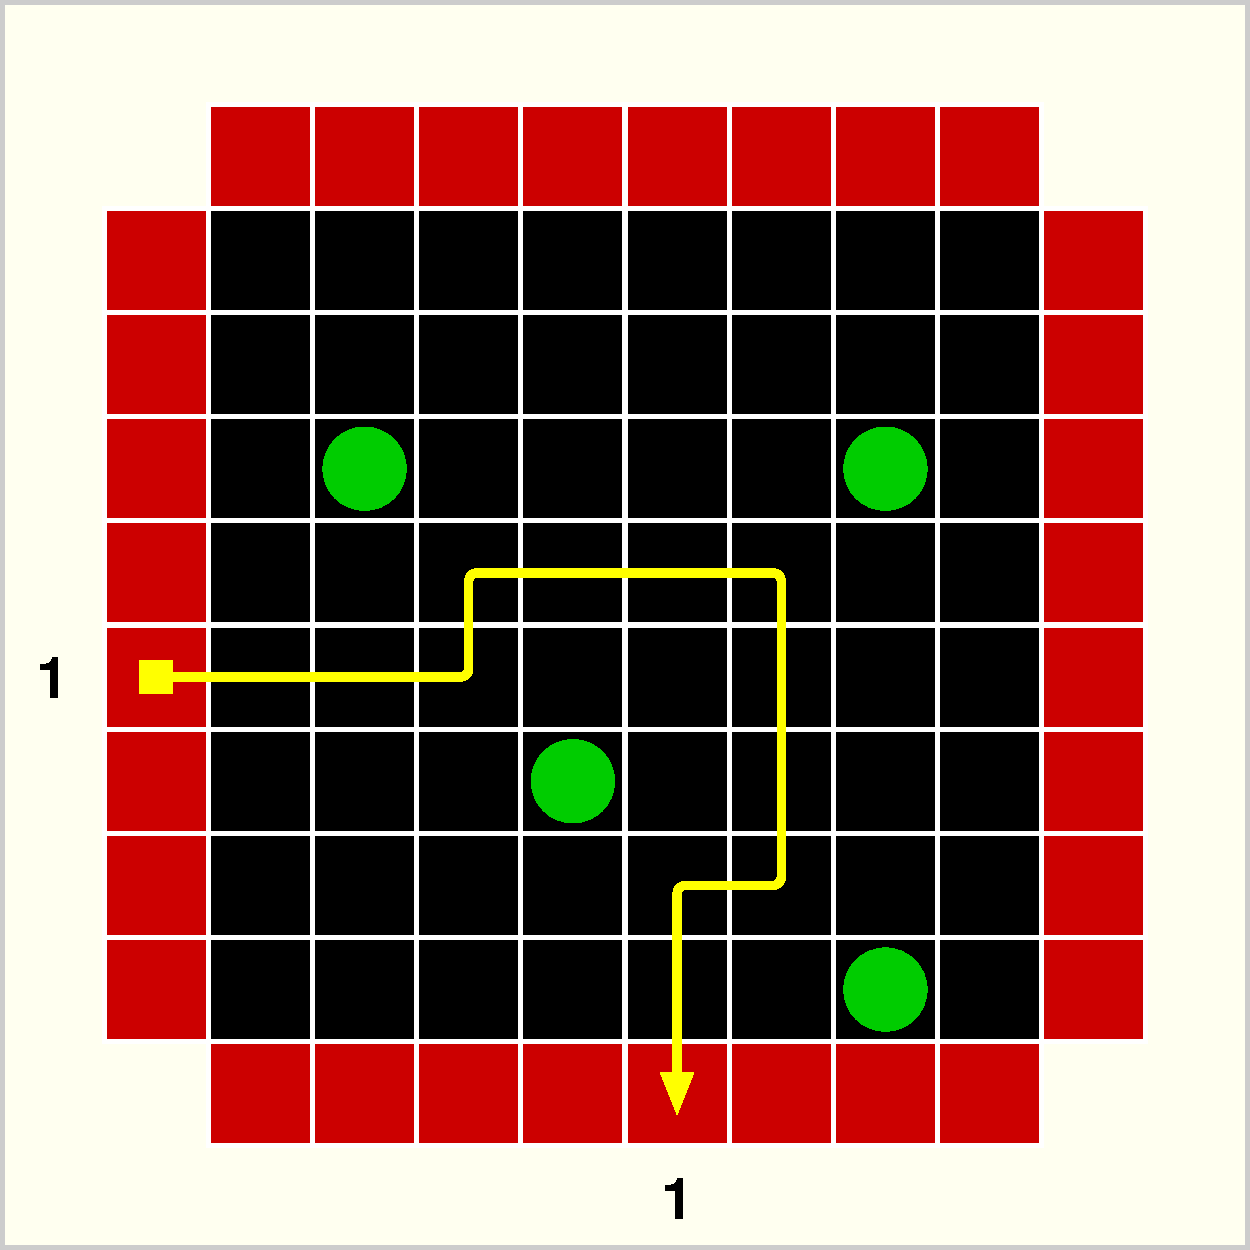
\includegraphics[width=\linewidth]{img/BlackBoxSample8.pdf}
    \vspace{-1em}
    \caption{Simple example, showing multiple deflections of a beam sent into the board.}
    \label{fig:deflection}
    \vspace{-1em}
\end{figure}
For detailed information about the rules of deflection, please visit the provided link in the footnotes. 
The single piece of information the opponent gets after each try is one of the following:
\begin{figure}[H]
    \centering
    \begin{tabular}{l l}
        \textbf{Hit} & The beam hit a ball directly \\
        \textbf{Deflection} & The beam exited somwhere else \\
        \textbf{Reflection} & The beam returned to the starting point
    \end{tabular}
\end{figure}
If the beam exits at some point different from the starting location, the opponent gets this point told. 
Based on the behaviour of these beams, the opponent has to deduce the position of the five balls.
Multiple deflections, reflections or just a pass through can occur, which makes the game so interesting. 
It is thus ultimately a puzzling game. 
The opponent can mark his guesses and submit a guess, if he has placed all five of them. 
He then gets told if it is correct or not, and eventually has to try until he finds the right configuration.
The scoring works as follows. 
\begin{figure}[H]
    \centering
    \begin{tabular}{l l}
        \textbf{Hit} & 1 Point \\
        \textbf{Deflection} & 1 Point \\
        \textbf{Reflection} & 2 Points \\
        \textbf{Submission} & 5 Points / Wrong Guess
    \end{tabular}
    \vspace{-1em}
\end{figure}
A lower score is better.
Average scores in the original board game range from 16 to 20.
The original game has also been adapted to different grid sizes, including 10x10 or 12x12 grid.
Our implementation therefore supports an arbitrary number of cells and balls.
% 
% 
\begin{figure}[t]
    \centering
    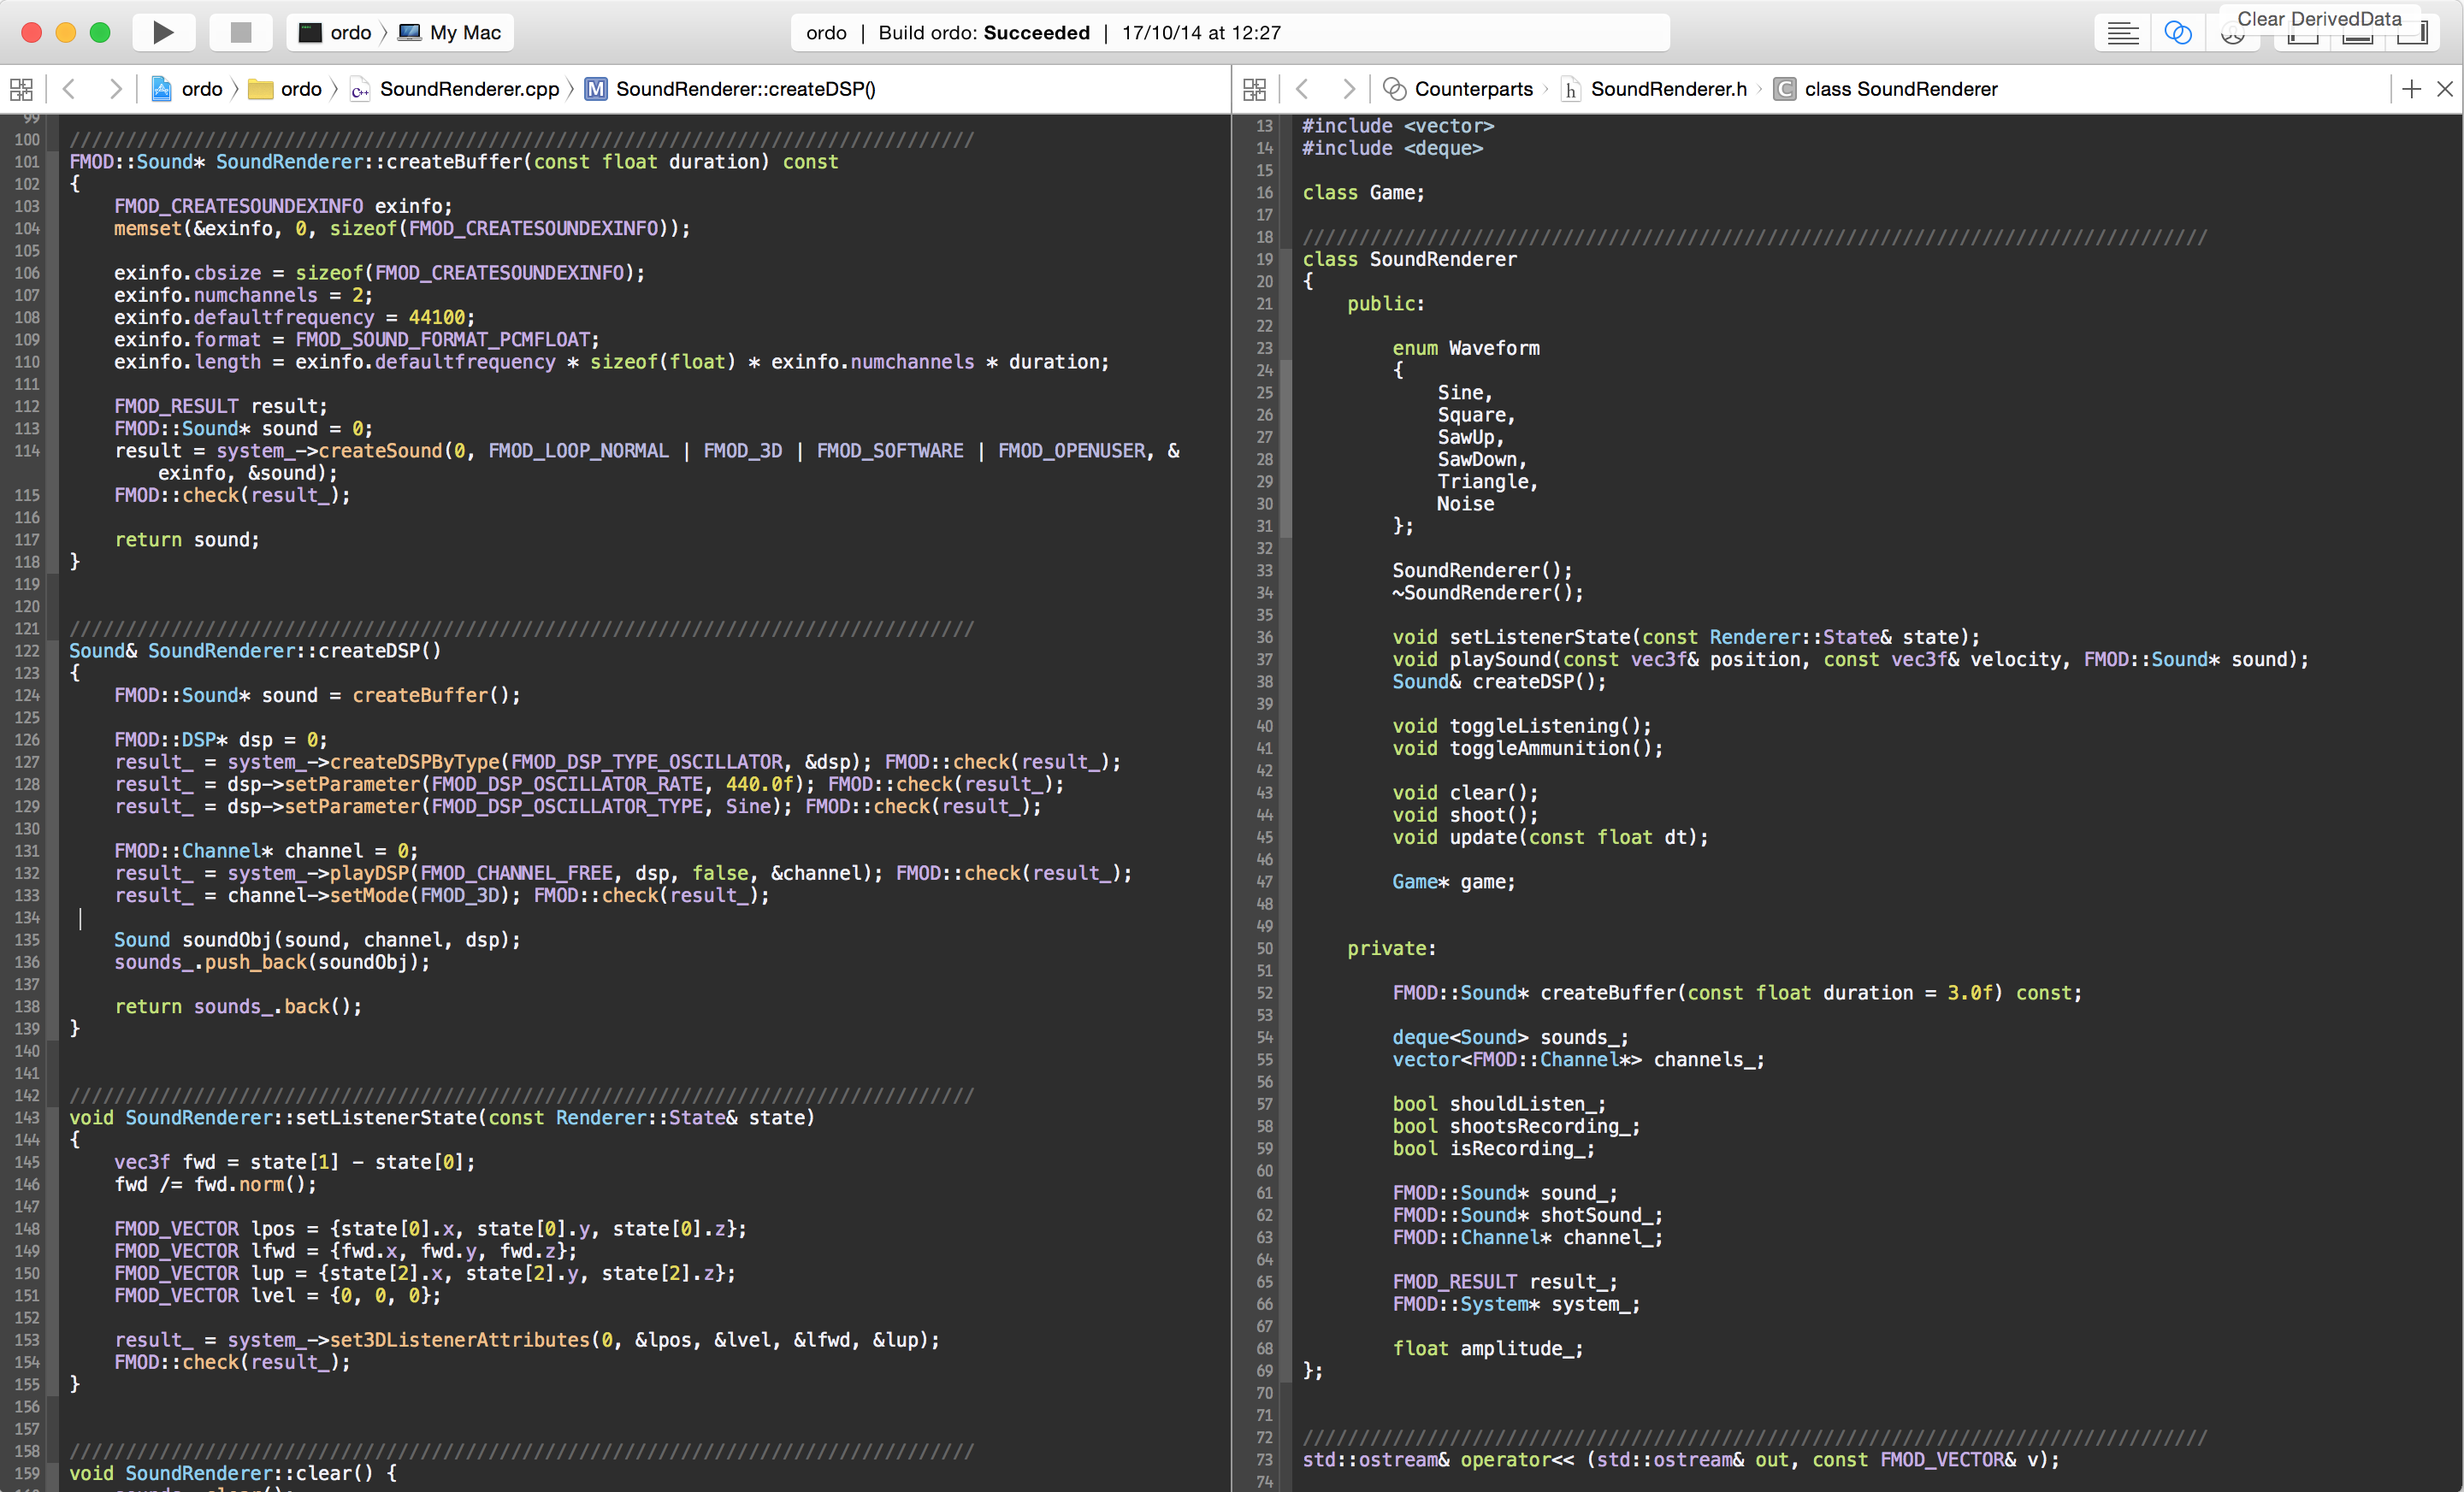
\includegraphics[width=\linewidth]{img/xcode_crop.png}
    \vspace{-1em}
    \caption{Impression of the working environement and excerpt of the \texttt{SoundRenderer} class.}
    \label{fig:xcode}
    \vspace{-1em}
\end{figure}
% 
% 
\section{Our Approach}
We took the concept of this game to a new level.
Instead of shooting imaginary light beams, the player shoots \textit{audio beams} into the world, which he is actually able to hear and follow. 
This implies, that the user needs to wear headphones and optionally has access to a microphone as input device.
We implemented different types of input.
The first one is triggered by pressing a key, which spawns a synthetic (i.e. sinusoidal) sound.
This sound is continuously playing, immediately starts traveling away from the player and moves through the field, influenced by the hidden balls.
The player has to listen and estimate its path, including current direction and all positions of deflection.
The player can also trigger a new beam by making a loud sound, e.g. snapping, clapping or shouting.
Finally, we wanted to go a step further and wanted to be able to use the input as feedback in the virtual world.
To this end, the user can make sounds and noises, which will then propagate through the field, replaying each time they make a turn.
% 
% 
\section{Implementation}
We implemented the game in \texttt{C++} using \texttt{OpenGL} and the \texttt{SFML}\footnote{\url{http://sfml-dev.org}} library for graphics and the \texttt{FMOD}\footnote{\url{http://www.fmod.org}} library for sound.
The latter is a professional audio library for high quality computation of spatial audio playback and effects. 
It also provides recording capabilities.
All audio is physically correctly rendered and emited through headphones.
\cref{fig:xcode} gives a brief impression of working environement and code design.
The basic game and audio logic was implemented in two days work, the graphics and interface took two more days, while the first complete gameplay including audio in- and output took another day.
All code has been made open source and is publicly available at \url{https://github.com/gurki/ardo}.
We tried to make the code clean, structured and readable.
However, as we tried to push forward more quickly and started experimenting, the current state, especially of the SoundRenderer class, has yet to be improved.
% 
% 
\section{Challenges}
One of the main questions from the beginning was how to handle microphone input.
We initially wanted to continously stream the audio input as a moving and almost living beam of sound.
To this end, we continously spawned new sound sources with the currently recording stream attached to it from the player's position. 
However, this led to an undifferentiable cloud of sound, which was not applicable at all.
We also encountered the problem, that in the current setting, only 64 sounds can be played at once.
Eventually, we thought about a different approach, where we automatically detect the user actively making input, by monitoring the amplitude level. 
When input is detected, a single sound is spawned, which travels into the field.
This sound has the current recording attached to it.
The twist now is, that it only plays, when it makes a turn, hits a ball or the border.
This approach led to a much clearer perception and was even more involving and fun, as the repeated playback creates a sort of suprise echoing effect from different locations.
We had beginning creating, copying and attaching different sound buffers to objects, which we could overcome in the end using the \texttt{FMOD} documentation and simple, restricted test cases.
% 
% 
\begin{figure}[b]
    \centering
    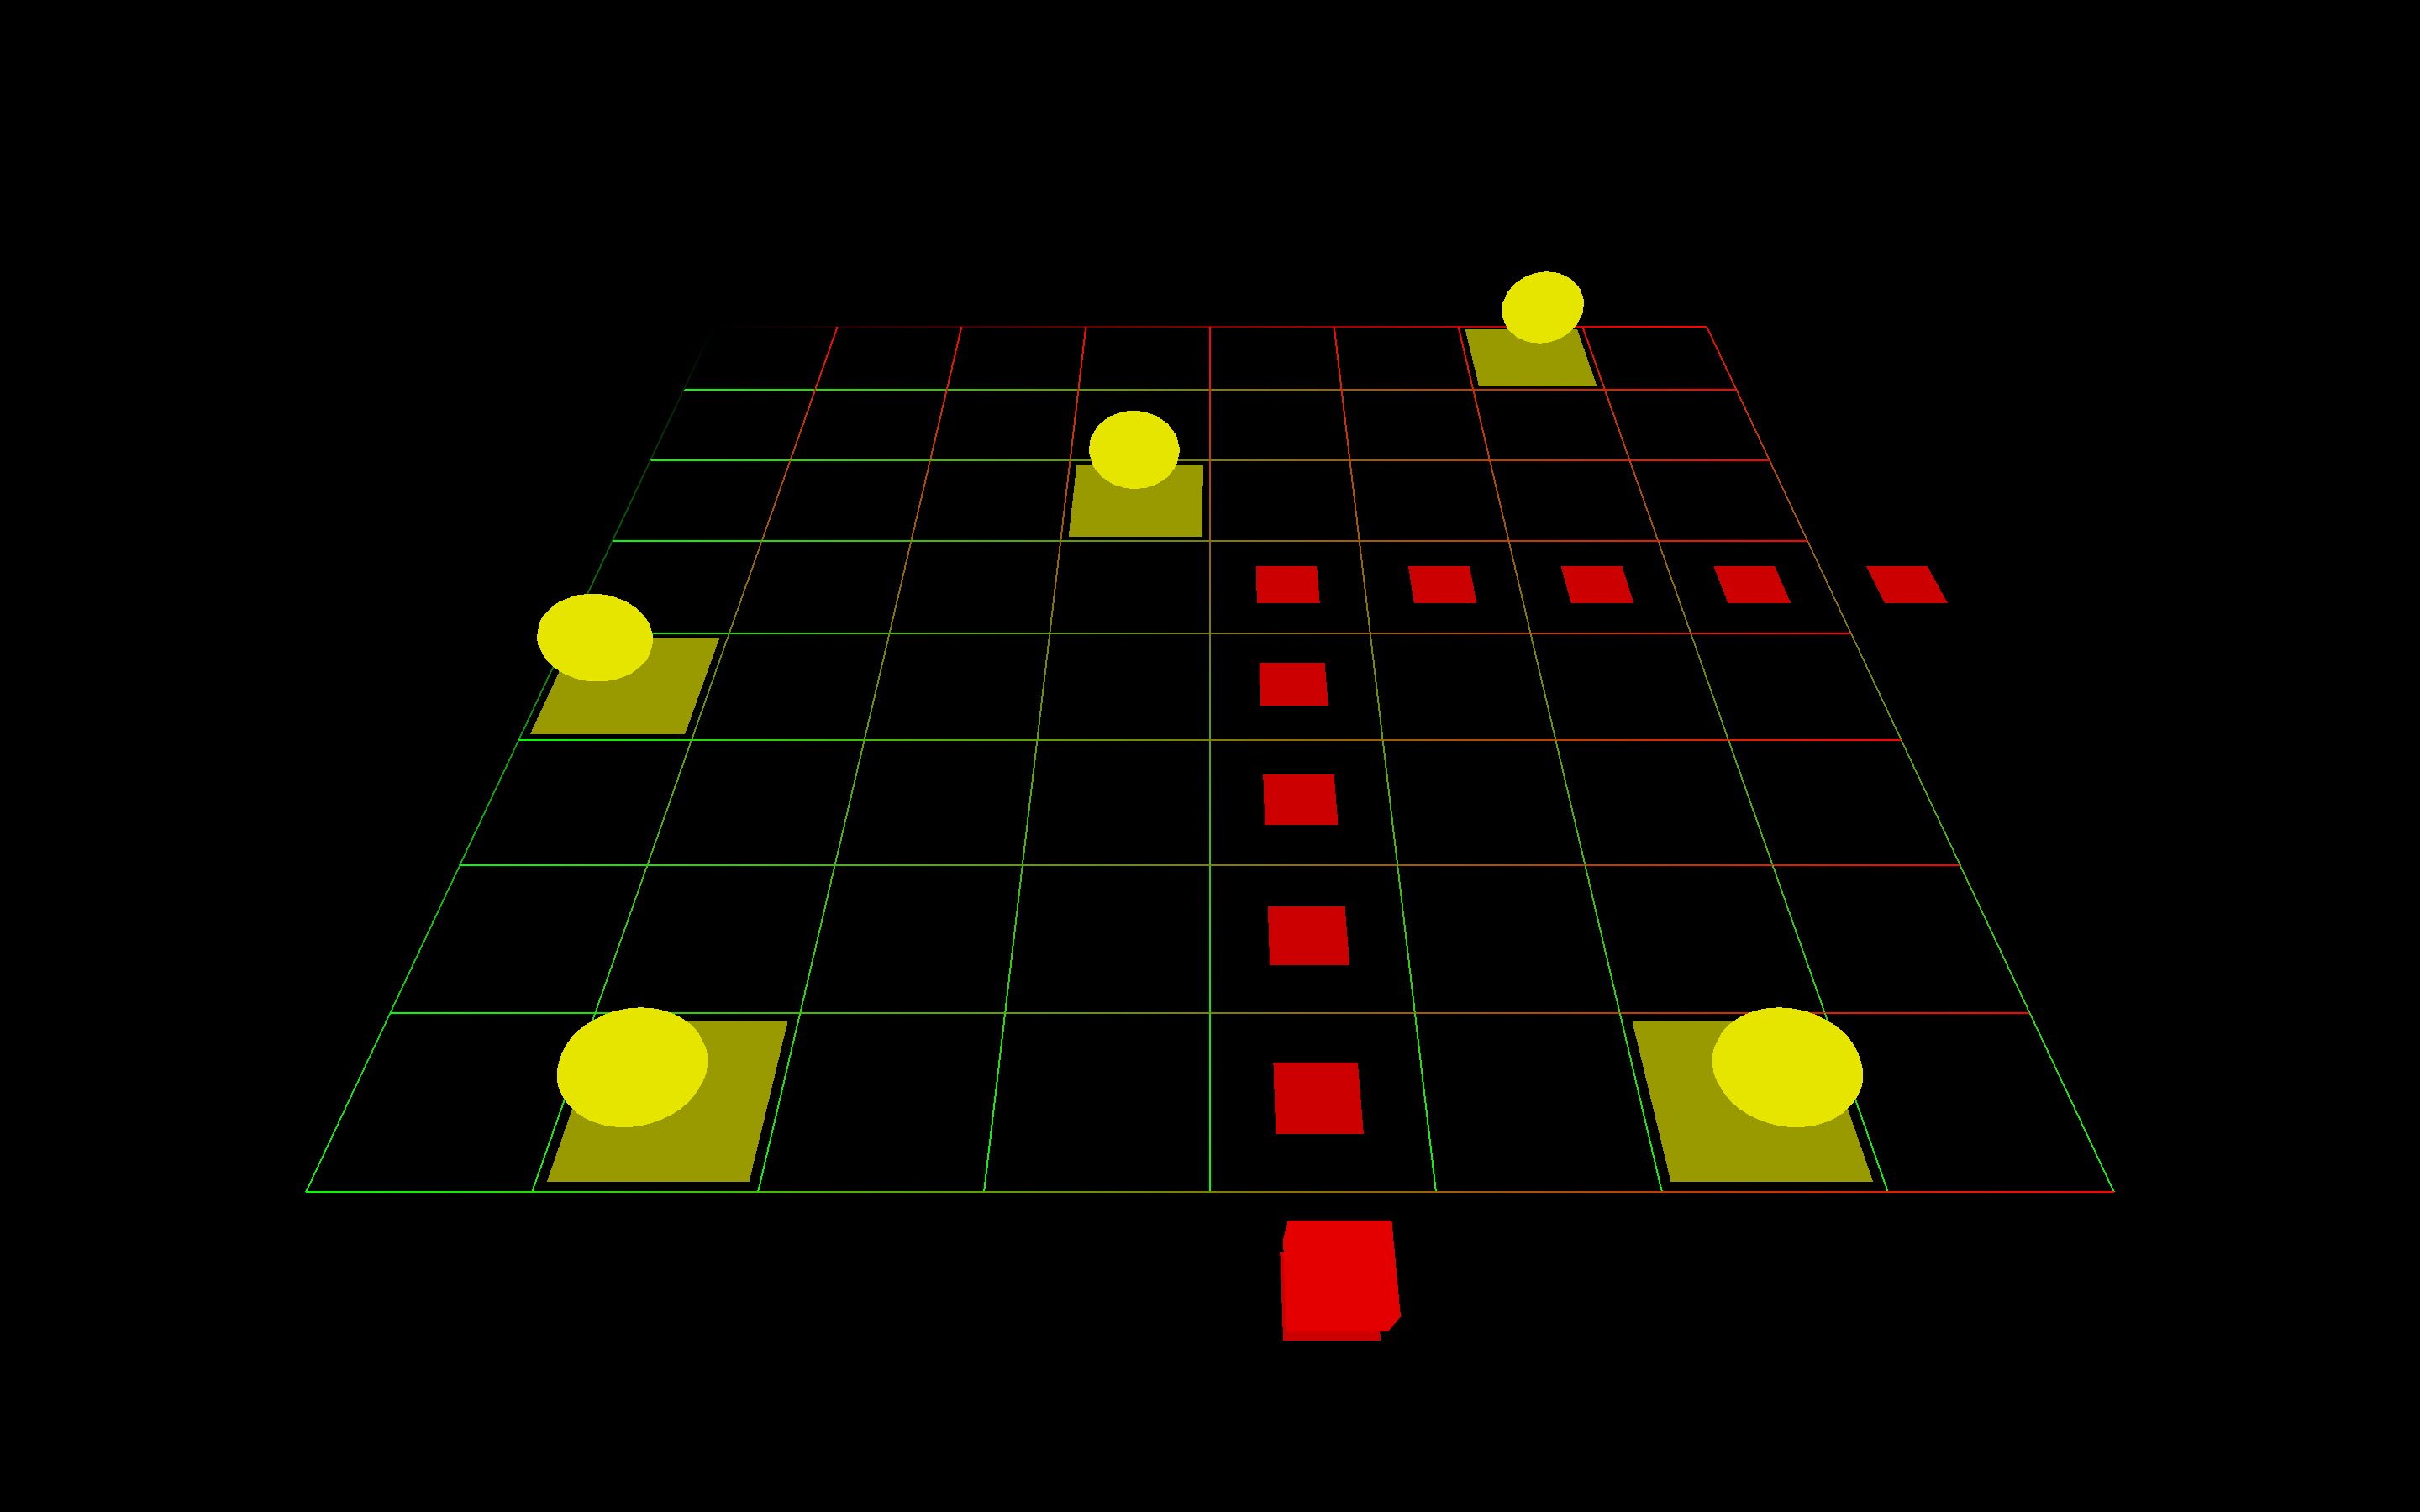
\includegraphics[width=\linewidth]{img/gameplay1.png}
    \vspace{-1em}
    \caption{Screenshot showing the board (grid), the five balls (yellow), the player (red cube) and the path the sound will take from the current position.}
    \label{fig:board}
    \vspace{-1em}
\end{figure}
% 
% 
\begin{figure*}[t]
    \centering
    \begin{subfigure}[t]{0.48\linewidth}
        \centering
        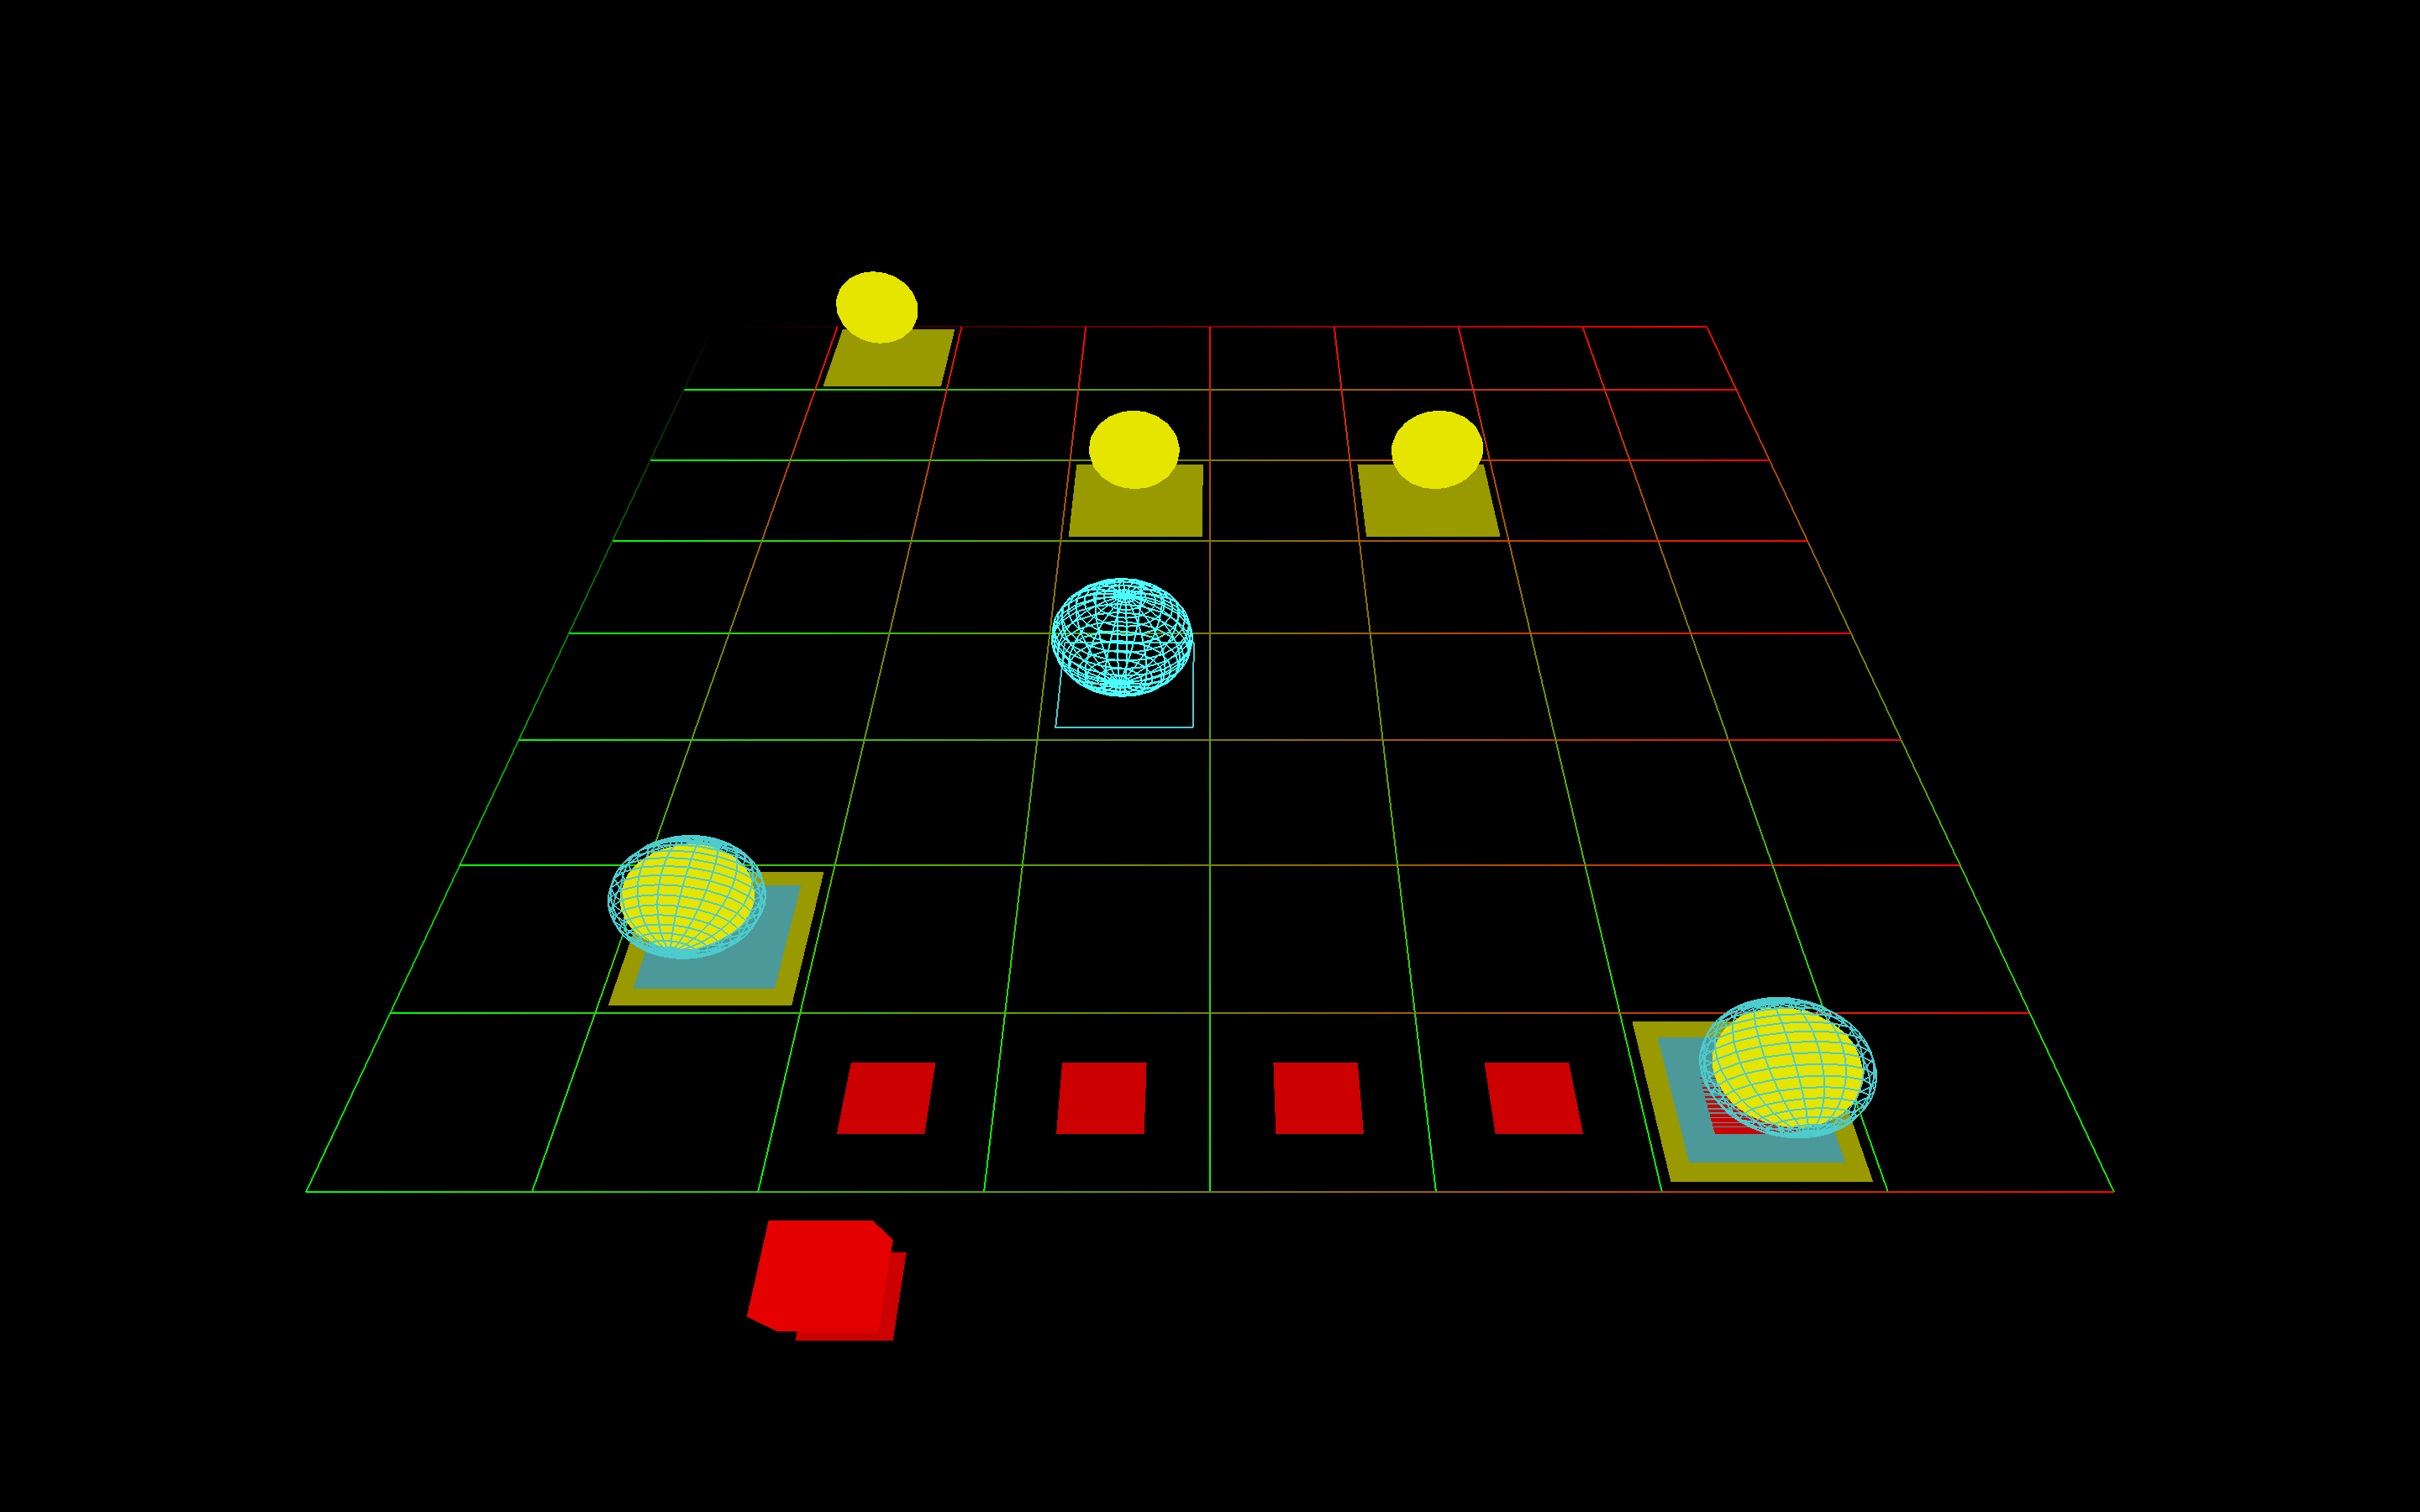
\includegraphics[width=\textwidth]{img/gameplay2.png}
        \vspace{-1em}
        \caption{Guess placing mode. The player can move the blue marker to set or erase his estimate of the hidden ball positions. For demonstration purpouses, the path and hidden balls are shown.}
        \label{fig:tpv}
    \end{subfigure}
    \hfill
    \begin{subfigure}[t]{0.48\linewidth}
        \centering
        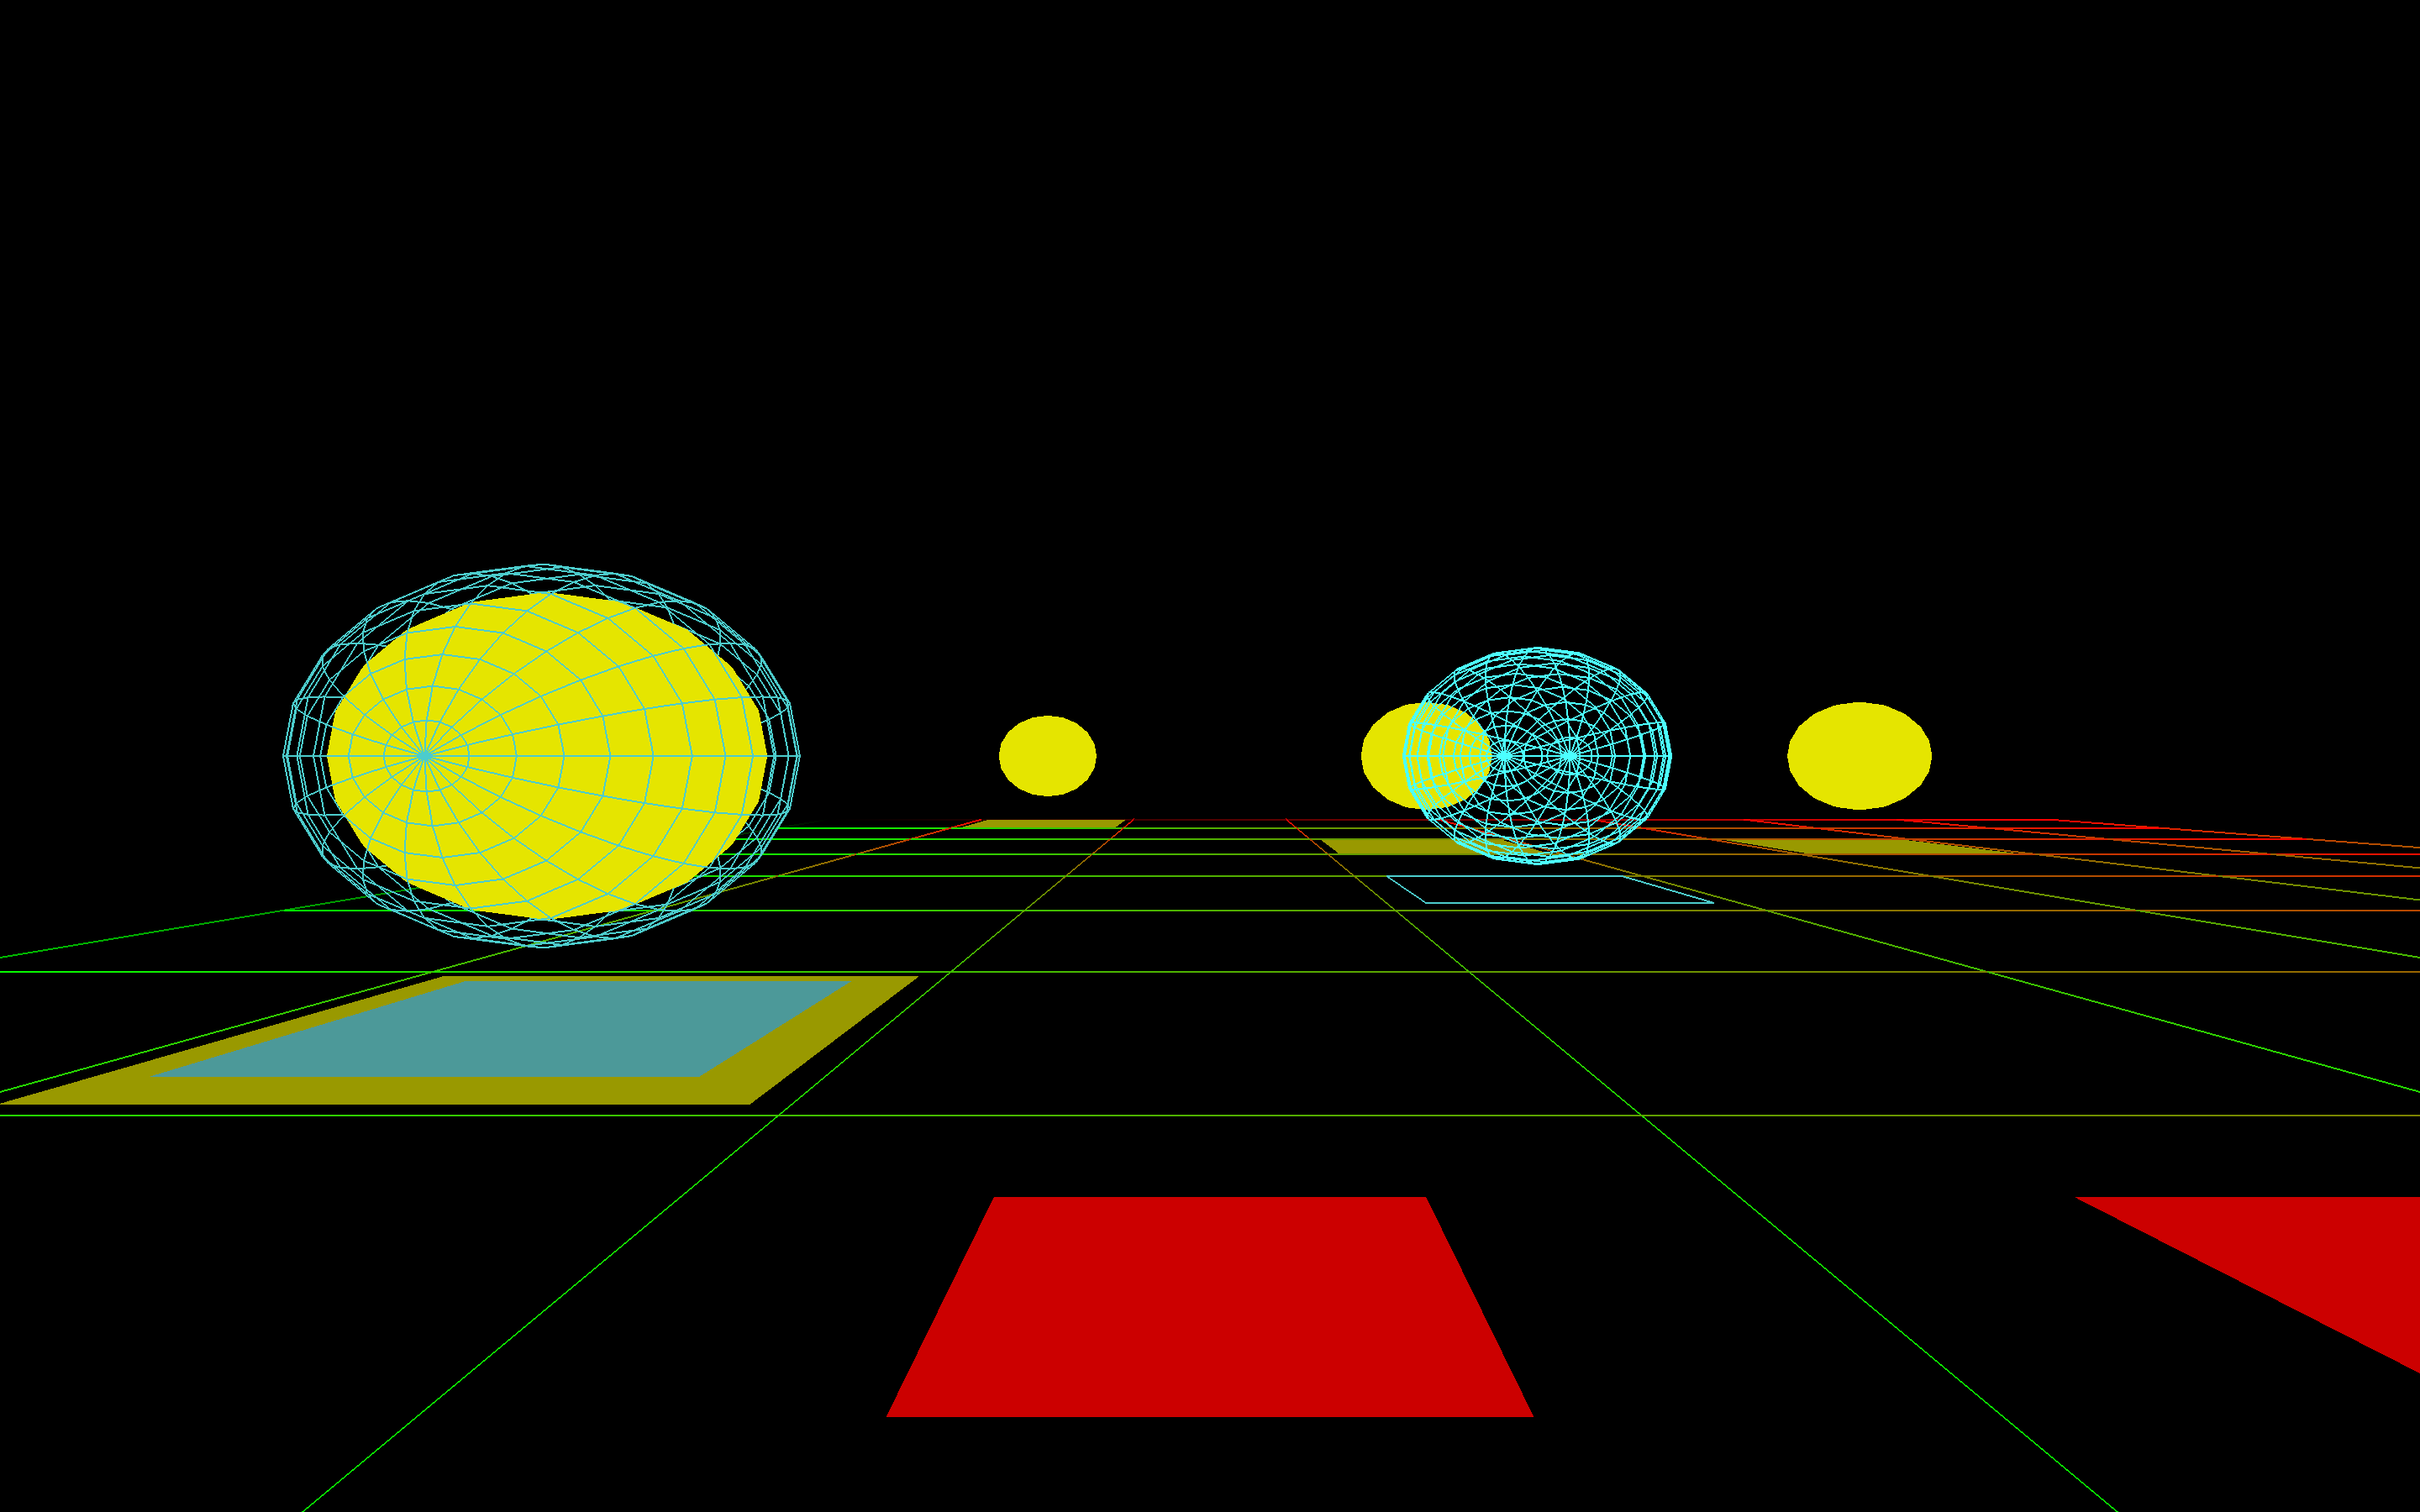
\includegraphics[width=\linewidth]{img/gameplay3.png}
        \vspace{-1em}
        \caption{(a) in first person mode. This is the actual perspective the game most time takes place in, as the sound is rendered according to the camera position. Note, that visualisations are turned off while playing.}
        \label{fig:fpv}
    \end{subfigure}
    \vspace{-1em}
    \caption{Bird eye and first person view of a scene.}
    \label{fig:views}
    \vspace{-1em}
\end{figure*}
% 
% 
\section{Results}
The game is fully playable as intended. 
\cref{fig:board,fig:views} show some in-game footage.
We aquired a group of ten participants to test our final application.
None of them knew the original game before.
We evaluated the following aspects. \\
\textbf{Simplicity.}
All participants understood the rules and how to play fairly quickly after we explained and showed some them example cases.
To discover the tricks and clues how to efficiently place beams and discover the balls took the participants two to three games on average.
Participants with previous video game experience performed better, as they got accustomed to the controls much more quickly and were thus less distracted during gameplay. \\
\textbf{Usability.}
As the game is in a very early stage and the focus was on the interaction using sound, the interface and controls are yet to be improved.
Currently, more then 10 keys are mapped to different functions, including moving around the board (\texttt{Left}, \texttt{Right}), activating different modes (e.g. \texttt{G} - Guessing, \texttt{I} - Toggle input, \texttt{V} - Toggle view) and placing guesses (\texttt{WASD} - Move marker, \texttt{Up} - Place, \texttt{Down} - Remove, \texttt{Enter} - Submit).
As mentioned, skilled video gamers could remember and handle the controls more quickly.
Other participants needed some time, but not more then one game, to adapt the controls.
Apart from that, once learned, all said that they find them quite convenient and the interaction enjoyable and fun. 
Especially our visualisitaion of placing guesses received positive feedback.
We also implemented a visual HUD to display important information as a quick introduction in the beginning of a game, current score or a mapping of keys.
This also was received positively. 
One problem has been presented by environmental factors.
For the microphone input to properly work, a too noisy environement had to be avoided.
We had some test cases, where the experience was hindered by background noise (library, seating group) triggering the recording or shooting of sounds. 
However, this was easily solved by moving to a more silent place. \\ 
\textbf{Difficulty.}
This was the most interesting point of our evaluations.
How well could one play the game just using sounds?
As it turns out, pretty well!
After a few minutes, the participants were able to more or less accurately make out the positions of the hidden balls.
The participants reported a very good sense of direction a sound was moving in, especially on the horizontal plane (left to right).
They also were able to make out movement away or towards them, but found it to be more difficult to qualitatively quantify the current distance to the ball.
This is of course to be reasoned with the physical structure of our hearing system (ears being on both sides of the head, not on the front and on the back).
We should however mention, that we found the movement of a pure sinusoidal sound itself quite challenging to estimate.
Before the evaluations, we thus added a percentual raise in pitch at every deflection or hit, which gives a much clearer indication to the player about movement and interaction with the balls.
When we switched to the recorded input mode, where sound is only repeated at hits or deflections, the recognition rate of the participants dropped noticably.
One reason is, that they first had to adapt and play around with the new form of input and feedback they got.
This however also coincides with the reports we got and predictions we made, that single sound locations are more difficult to estimate than continously moving streams. \\
\textbf{Enjoyability.}
Nevertheless, the motivation of the participants was even higher in this more involving mode, as it was reported to be very funny and interesting to listen to his own voice bouncing and travelling through the field.
We also received comments, that participants had fun trying different sounds and levels of loudness to find the one sound, that works optimally.
Even in the synthesised sound setting, users seemed to enjoy the experience and gameplay, as most of them requested to play more then two rounds.
% 
% 
\section{Discussion}
We are pretty satisfied with our results.
We achieved our initial goals and were able to present a working version of ARDO, the Audio-ORDO using sound as main gameplay feature.
Our evaluations show, that spatialised sound can be used to estimate the position of landmarks in a virtual 3D world.
They also show, that sound as main input and output is a enjoyable and refreshing new way to interact in a video game.
The game is fully playable and coherent as it is. 
However, for now this is only a protoype.
There are several things we could and eventually will improve or add.
Firstly, the graphics could be improved, as this was not the focus of this work.
Furthermore, we could explore other game modes. 
For example, the player could be able position static beams on the field that would stay in place and continue to produce sound.
This pipe of sound could be experienced by moving around the field, in contrast to moving only on the borders.
The player would have to find the balls before the board is too crowded with noise. 
We also thought about adding a harder mode, where only the final position would be sonified, thus bringing our interpretation of the game closer to the original, where you’re only told where the path ended.
Ultimately, we plan an actual two player version, which could be played online in the browser.
The starting player could listen to the input of his opponent and even interfere by making countersounds, that alter the behaviour of the board.
% 
% 
\bibliography{bibliography.bib}
\bibliographystyle{plain}
% 
\end{document}